% !TEX root = writing_version.tex

\label{chp:theory}

%\section{Markovian assumption and the nucleation rate discrepancy}
\section{Introduction}
\label{sec:memory_approach}
Understanding and describing phase transitions has always been as important as it has been challenging. On the one hand, its importance can be seen in technological disciplines like metallurgy or in scientific fields like atmosphere physics. Metal melts, for example, will form different grain sizes depending on how fast they solidify. The need for an accurate description of phase transitions then becomes obvious when considering that the grain size is crucial for properties like rigidity and brittleness. On the other hand, the challenge is due to the large number of participating particles which make an exact description impossible.\\

Nevertheless, a concept to qualitatively describe phase transitions was developed early on. Today, this is called classical nucleation theory (CNT). In it, a free energy is defined for some collective observable which describes the transition. This free energy landscape includes a barrier separating the two distinct phases and starting from the unfavorable phase, the system will eventually cross the barrier due to thermic Markovian fluctuations. The average duration of this process is called induction or nucleation time and usually is determined by the temperature and the barrier height.\\

\subsection{Testing the Markovian assumption}
In \autoref{sec:CNT}, CNT is discussed in more detail. Also, it is used a few times within this thesis. However, it has been shown by Sear 2012\cite{Sear2012} that in many circumstances the approach fails to provide a quantitative description. As this is not only unsatisfying for a theorist, but actually of importance in many fields of science, various approaches to solve this problem have been proposed in the past. A comprehensive list of them can be found by Kuhnbold et al. 2019\cite{Kuhnbold2019}. The list includes modifying the free energy landscape, choosing suitable reaction coordinates or to include non-Markovian effects in the description.\\ 

In the article by Kuhnbold et al., the presence of the latter is illustrated for the largest cluster in the metastable Lennard-Jones system. Similarly Pelagejcev 2019\cite{ThesisPhilipp} found non-negligible memory kernels in the same system by employing a numeric memory kernel reconstruction scheme which was derived by Meyer et al. 2019\cite{Meyer2019a}. In this thesis, we will continue to extend the examples of memory kernel studies by adding our findings in the elastic hard sphere system in \autoref{sec:memory_kernels}.\\

While the theory and framework to obtain the non-stationary memory kernel is too broad to cover at this point, we may mention the foundations as given by Meyer 2020\cite{MeyerThesis} in his dissertation.\\

In the 1960's Mori and Zwanzig used their projection operator formalisms to show that memory effects can a priori not be excluded for the time evolution of collective observables. Within these formalisms, the generalized Langevin equation (GLE) was derived and later on Grabert developed a time dependent formalism to include non-stationarity. Based on these earlier works, the non-stationary generalized Langevin equation was derived by Meyer et al. 2017\cite{Meyer_nsGLE}. It is the equation of motion for a coarse grained observable $A$ and is given by
\begin{equation}
\label{eqn:EOM_A}
  \frac{d A_{t}}{dt} = \omega (t) A_{t} + \int_{0}^{t} K(\tau, t) A_{\tau} d\tau + \eta_{0,t} \; \text{.}
\end{equation}
In the equation, $A_{t}$ denotes the observable which depends on the time $t$ for a specific trajectory, $\omega (t)$ is the time dependent friction coefficient, $\eta_{0,t}$ is the time dependent noise term and $K(\tau, t)$ is the memory kernel depending on two times. From the structure, we see that the kernel holds the information on how the observable's history influences its future. Moreover, we see that the equation is fully time dependent to suit the description of non-stationary processes like phase transitions. For purely Markovian and stationary processes, we expect to find a Dirac delta distribution, as no memory is present. In this case, \autoref{eqn:EOM_A} simplifies to the usual Langevin equation.\\

\subsection{Studying the nucleation rate discrepancy}
While the study of memory effects is one major aim of this thesis, the other one is to measure nucleation rates of the metastable hard sphere fluid. They are an active topic of research, as those from laboratory based experiments and those from numerical simulation studies differ by orders of magnitude. See for example Auer and Frenkel 2001\cite{Auer2001}, Filion et al. 2010\cite{Filion2010a}, Schilling et al. 2011\cite{Schilling2011}, Wood 2019\cite{Wood2019} or Fiorucci et al. 2020\cite{Fiorucci2020a}. To shed some light on the problem, a detailed analysis and characterization of the nucleation process is done. This leads to a possible remedy of the discrepancy as is discussed in \autoref{sec:inf_vol_limit_nuc_rate}.
\newpage

\section{The hard sphere system}
\label{sec:HS_system}
The hard sphere system is the simplest model of a fluid which goes beyond the ideal gas only by including interactions between the particles in the form of an occupied volume. Its potential between particles $i$ and $j$ is given by
\begin{equation}
\label{eqn:hs_potential}
V(r_{ij})=%\infty \cdot \Theta(\sigma - r_{ij})
\begin{cases}
\infty \quad & r_{ij} \le \sigma \\
0 \quad & r_{ij} > \sigma
\end{cases} \; \text{.}
\end{equation}
In this equation, $r_{ij} = |r_j - r_i|$ denotes the distance between the two particles and $\sigma$ is the diameter of a hard sphere.\\

While the ideal gas model without pair interactions already makes it possible to derive the famous equation of state $pV=NkT$, it does not include phase transitions yet. Those can be observed when granting the particles to occupy space, in the simplest case, by defining hard spheres of the kind in \autoref{eqn:hs_potential}. As it is the simplest model and it is efficiently accessible for computer simulations, the hard sphere system is very well suited to study basic properties of first order phase transitions.\\ 

The first hard sphere computer simulation dates back to the beginning of electronic computer technology, in first studies by Alder and Wainwright in 1959\cite{Alders59}. Since then, more algorithms have been elaborated to increase efficiency and technology has advanced to a point at which virtual studies of large systems of the order of one million particles become tractable. Hence, computer simulations are becoming an even more powerful tool to study phase transitions of simple systems.\\

Nevertheless, even large computer simulations are very constrained in their size in comparison to laboratory based experiments, where similar systems are realizable and extensively studied. But in simulations, general properties of the system at hand can be varied effortlessly and information about each single particle can be extracted as they are naturally required. Therefore, the possibilities to analyze these virtual systems are larger than in the laboratory systems.
\section{The hard sphere phase diagram and its metastable state}
\label{sec:HS_phase_diagram}
The equation of state for the monodisperse hard sphere system has various parametrizations as, for example, listed by Mulero et al. 2001\cite{Mulero2001}. The most common of them, due to its simplicity, is the approximation proposed by Carnahan and Starling 1969\cite{Carnahan1969}, given by
\begin{equation}
\label{eqn:CS}
Z=\frac{1+\eta+\eta^2-\eta^3}{(1-\eta)^3} \; \text{.}
\end{equation}
It approximates the compressibility factor Z as a function of the packing fraction $\eta$ for the hard sphere fluid.\\

Similarly, many approximations exist for the equation of state on the stable solid branch. A common one is given by Almarza 2009\cite{Almarza2009}. It is parameterized as
\begin{equation}
\frac{p(v-v_0)}{k_B T} = 3 - 1.807846 y + 11.56350 y^2 + 141.6 y^3 - 2609.26 y^4 + 19328.09 y^5 \; \text{.}
\end{equation}
In this equation, $p$ is the pressure, $v$ is the volume per particle, $v_0=\sigma^3/\sqrt{2}$ is the volume per particle at close packing and $y=p \sigma^3 / (k_B T)$, with $k_B$ being the Boltzmann constant, $T$ the temperature of the crystal and $\sigma$ the diameter of the spheres.\\
We may note, that the inverse of the volume per particle corresponds to the number of particles per volume $ v^{-1} = \rho$. The relation to the corresponding packing fraction $\eta$ is given by $\rho = \frac{6}{ \pi} \eta$, which can be easily shown by extending $\rho = \frac{N}{V}$ by the single particle's volume $V_s = \frac{4}{3} \pi \left(\frac{\sigma}{2}\right)^3 = \frac{\pi}{6} \sigma^3$.\\
%Within the thesis mostly but not only the volume fraction is used as it is the most common parameter for describing the hard sphere system, but it can always be exchanged by the density.\\ 

A first order phase transition is observed when switching between the two stable branches of the system, described by the two equations of state, between volume fractions of $\eta_{\text{freeze}} = 0.494$ and $\eta_{\text{melt}}=0.55$. The freezing volume fraction corresponds to first solidifying clusters when approaching the transition from the liquid branch. Accordingly, the melting volume fraction indicates the melting of the crystalline phase when approaching the transition from the solid branch. Within this interval, the system tends towards a coexistence state which in equilibrium varies by the fraction of solid to liquid volume.\\
In detail, the liquid may follow its branch to pressures above the coexistence pressure where it becomes unstable. The particles then rearrange into the crystalline phase as each single particle can access a larger volume in the structured lattice than it would be possible in the unordered fluid.\\
This becomes evident by comparing the volume fractions of random close packing $\eta_{\text{RCP}}\approx 64\%$ with the one of a face centered cubic or hexagonal close packing fraction of $\eta_{\text{HCP}} \approx 74 \%$. Within the crystalline phase each particle still has free accessible volume, while the randomly packed particles are already confined at exactly one place.\\
The additional accessible volume translates into a larger number of possible states for the particle or in terms of thermodynamics, a larger entropy which acts as a driving force for the phase transition. As the particles in the crystal are packed more densely with a volume fraction of $\eta_{\text{melt}}=0.55$, the pressure is reduced and not all fluid transforms into the solid phase, but both phases may coexist.\\

The overall phase diagram is shown with the coexistence pressure in \autoref{fig:hs_phase_diagram}.\\

\begin{figure}[h]
\centering
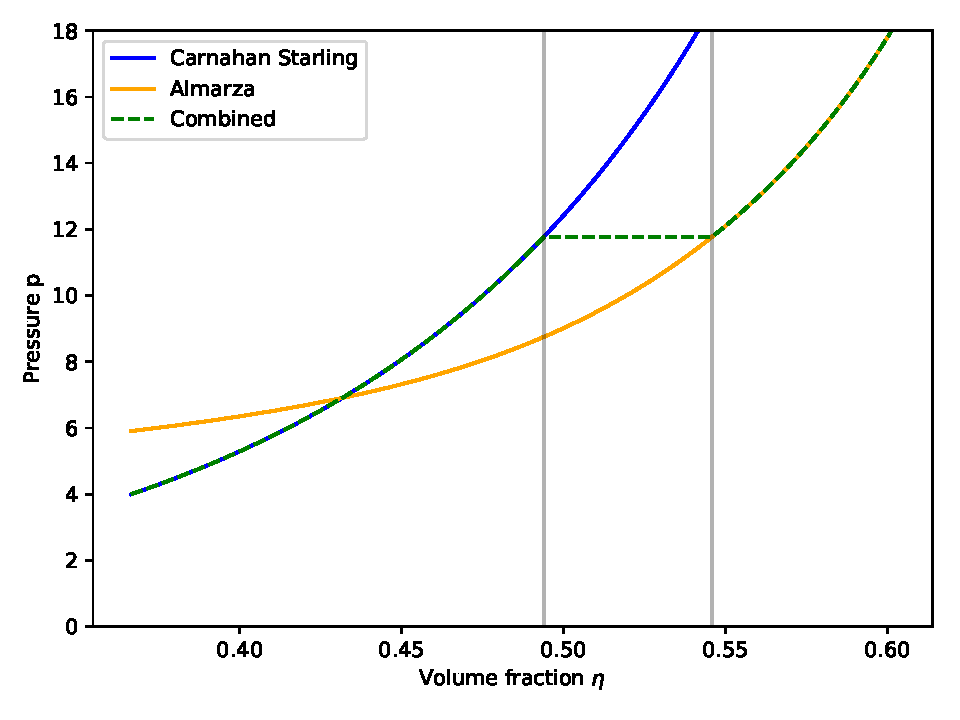
\includegraphics[width=0.65 \linewidth]{Hard_sphere_phase_diagram.pdf}
\caption[Phase diagram of hard sphere fluid]{Phase diagram of the hard sphere system with freezing and melting volume fraction shown as shaded lines and the green dashed line indicating the equilibrium stable branch. Where liquid and solid branch do not coincide with the stable branch, systems are unstable and tend towards a state on the stable branch.}
\label{fig:hs_phase_diagram}
\end{figure}
\FloatBarrier
The equilibration solid fraction of the system, $x_s = \frac{V_s}{V}$ with $V_s$ the solid volume and $V$ the total volume, are described by \autoref{eqn:solid_fraction_result}.\\ 
For the derivation it is necessary to keep in mind that, in the stationary coexistence state, the density of the solid phase is given by the melting density and that the liquid density is equal to the freezing density, i.e $\rho_s = \rho_{\text{melt}}$ and $\rho_l = \rho_{\text{freeze}}$ respectively. When further using the trivial equations
\begin{align}
V &= V_s + V_l \; \text{,} \nonumber\\
N &= n_s + n_l \; \text{,} \nonumber\\
N_i &= \rho_i V_i \; \text{,} 
\end{align}
with $n_{\text{s/l}}$ the number of solid/liquid particles we may write
\begin{align}
\rho V &= \rho_s V_s + \rho_l V_l \; \text{.}
\end{align}
Under the assumption of equilibrium it leads, within a few lines of calculation, to 
\begin{align}
\frac{V_s}{V} &= \frac{\rho - \rho_{\text{freeze}}}{\rho_{\text{melt}} - \rho_{\text{freeze}} } \; \text{.}
\end{align}
As the solid fraction below $\rho_{\text{freeze}} $ vanishes and above $\rho_{\text{melt}}$ is 1, we can conclude that the equilibrium solid fraction of the system is given by \autoref{eqn:solid_fraction_result}.
\begin{align}
\label{eqn:solid_fraction_result}
x_s(\rho) = 
\begin{cases}
0 & \rho <  \rho_{\text{freeze}}\\
\frac{\rho-\rho_{\text{freeze}}}{\rho_{\text{melt}}-\rho_{\text{freeze}}} &  \rho_{\text{freeze}} < \rho <  \rho_{\text{melt}}\\ 
1 &  \rho > \rho_{\text{melt}} \quad \quad \text{.}
\end{cases}
\end{align}

Evaluating \autoref{eqn:solid_fraction_result}, between volume fractions of $\eta \in [0.53,0.55]$, leads to coexistence fractions of $x_s \in [0.7,1]$. This means that we are expecting nucleated systems in simulations to consist mostly of the solid phase after enough time for complete crystallization.\\

As pointed out earlier, the phase transition takes place as it reduces the pressure in the liquid. This means that already during the growth of clusters the volume fraction of the metastable liquid is reduced, potentially altering its behavior significantly. For closer inspection of this, the particle density of the metastable liquid depending on the solid fraction $x_s$ is evaluated in \autoref{eqn:meta_stable_volume_fraction}. For this purpose, first, the liquid volume $V_l$ and the number of liquid particles $N_l$ are expressed in terms of the solid fraction $x_s$:
\begin{align}
\label{eqn:volume_relation}
V_l(x_s) & = V(1-x_s)\\
\label{eqn:number_relation}
N_l(x_s) & = N-n_s(x_s) = N - \rho_m V x_s = N(1-\frac{\rho_m}{\rho}x_s)
\end{align}
Combining \autoref{eqn:volume_relation} and \autoref{eqn:number_relation} to the expression for the particle density in the remaining liquid leads to
\begin{align}
\label{eqn:meta_stable_volume_fraction}
\rho_l(x_s) &= \frac{N_l (x_s) }{ V_l(x_s) } = \frac{N}{V} \frac{1-\frac{\rho_m}{\rho}x_s}{1-x_s} = \rho \frac{1-\frac{\rho_m}{\rho}x_s}{1-x_s} \; \text{.}
\end{align}
 
Evaluating the expression for relevant volume fractions within $\eta \in [53\%, 55\%]$ leads to the conclusion that crystalline fractions of $x_s < 5\%$ only reduce the packing fraction in the fluid by 0.1\%. Especially for system sizes of about 1 million particles, this already corresponds to cluster sizes of a few ten thousand particles where stable growth of clusters takes place which is rather insensitive to changes of the volume fraction as shown in \autoref{sec:cluster_growth}. This shows, that during the highly sensitive cluster forming processes the volume fraction of the liquid can be assumed to be globally stable.

\section{Classical nucleation theory }
\label{sec:CNT}
Classical nucleation theory (CNT) has been proposed by Becker and Döring in 1935\cite{Becker1935} and since then used and modified multiple times to suit various types of systems. It still provides some reference or expectation, even if its framework does not seem to encompass the full nucleation process, to compare with the simulation data.\\

The simplest version of CNT assumes that a spherical crystallite of radius $R$ may form in the liquid with properties of the bulk crystal, while the fluid remains with the properties of the bulk fluid. The difference in the free energy landscape is given by a surface and a volume term, each depending on the radius. The first arises from the surface tension $\gamma$ between the fluid and the solid bulk phase, while the latter is caused by the difference in chemical potential $\Delta \mu$ between the two phases. The whole expression for the free energy is given by
\begin{equation}
\label{eqn:free_energy}
\beta \Delta G(R) =4 \pi R \gamma -\frac{4}{3} \pi R^3 \rho \Delta \mu  \; \text{,}
\end{equation}
with $\rho$ being the particle density of the solid phase.\\

To calculate the difference between the chemical potentials $\Delta \mu $, we first derive the free energy difference between the metastable liquid branch and the stable coexistence branch. To calculate the free energy, we employ its differential relation
\begin{align}
\label{eqn:differential_relation}
dF = -S  \, dT -P \, dV + \mu  \, dN \; \text{.}
\end{align}
Setting the number of particles and the temperature constant and further reformulating $dV$ using \linebreak[1] $dN = dV  \, \rho + V  \, d\rho  $ and $dN = 0 $, we find $ dV = -d\rho \frac{N}{\rho^2}$. Under this transformation, \autoref{eqn:differential_relation} becomes
\begin{align}
\label{eqn:df_relation}
\frac{dF}{N} = \frac{P(\rho)}{\rho^2} d\rho \; \text{.}
\end{align}

The pressure $P(\rho)$ is approximated by the Carnahan-Starling equation of state where we use $\eta = \frac{6 \rho }{\pi}$ and $Z=\frac{pV}{NkT} = \frac{p(\rho)}{\rho kT}$. Hence, the integration of \autoref{eqn:df_relation} between two densities $\rho_{1/2}$ is given by
\begin{equation}
\frac{\Delta F}{N} = \int_{\rho_1}^{\rho^2} \frac{kT}{\rho} \frac{1+\left( \frac{6 \rho}{\pi}\right) +\left( \frac{6 \rho}{\pi}\right)^2 - \left( \frac{6 \rho}{\pi}\right)^3}{\left( 1 - \frac{6 \rho}{\pi}\right)^3} d\rho \; \text{,}
\end{equation}
with the analytical solution
\begin{equation}
\int_{x_1}^{x_2} \frac{1+(ax) +(ax)^2 - (ax)^3 }{( 1 - ax )^3 \,  x} dx = \left. \frac{3-2ax}{(ax-1)^2} + \text{log}(x) \right|_{x=x_1}^{x_2} \; \text{.}
\end{equation}
Dropping the lengthy notation for $\eta$ we end up with
\begin{equation}
\frac{\Delta F}{N} = kT \left(  \frac{3-2 \eta_2}{(\eta_2 - 1)^2} - \frac{3-2 \eta_1}{(\eta_1 - 1)^2} + \text{log}\left( \frac{\eta_2}{\eta_1} \right) \right) \; \text{.}
\end{equation}
The analytical solution is compared in \autoref{fig:free_energy_diff} with numerically results which have been calculated before the analytical solution was found. In the following, the free energy difference is identified with the difference in chemical potential $\Delta \mu$ as it is the driving force of the nucleation.\\

\begin{figure}[h]
\centering
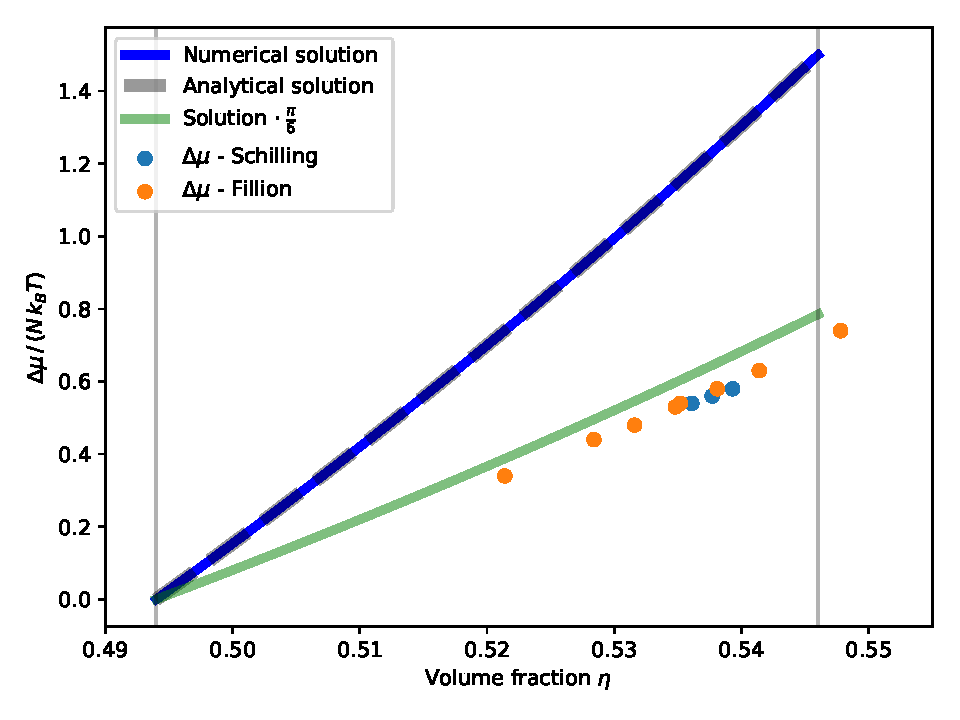
\includegraphics[width=0.53 \linewidth]{Free_energy_difference.pdf}
\caption[Free energy difference between fluid and solid phase]{Free energy difference per particle between the metastable liquid phase and the coexistence phase. Values by Schilling et al. 2011\cite{Schilling2011} and Filion et al. 2010\cite{Filion2010a} deviate from the shown result, but we assume that a factor of $\frac{\pi}{6}$ in the calculations is missing in either this or their calculation, as the modified green curve collapses rather accurately on the literature values when choosing $\eta_{\text{freeze}}=0.5$.}
\label{fig:free_energy_diff}
\end{figure}

Coming back to the free energy landscape of \autoref{eqn:free_energy}, we see that it exhibits a maximum at a radius called $R_{\text{crit.}}$. The interpretation of this radius is, that if a cluster surpasses the critical radius it is likely to keep growing until the system settles at the equilibrium solid fraction. Here, a cluster is defined as a structure having a locally crystalline like ordering. The critical radius, simply calculated by setting the derivative of \autoref{eqn:free_energy} to zero, is given by
\begin{equation}
\label{eqn:r_crit}
R_{\text{crit.}} = \frac{2 \gamma}{\rho \Delta \mu } \; \text{,}
\end{equation}
and the height of the barrier at the critical radius is given by
\begin{equation}
\beta \Delta G (R_{\text{crit.}}) = \frac{16 \pi \gamma^3}{3 \rho^2 (\Delta \mu )^2} \; \text{.}
\end{equation}

The classical critical radius depending on the volume fraction is depicted in \autoref{fig:r_crit} for a first impression of the cluster sizes that we are expecting for nucleation. The interfacial surface tension for this often is given by $\gamma \approx \SI{0.6}{k_B T \sigma^{-2}}$, but its precise value is under debate. Thus, we may stick to one of the recently calculated values of $\gamma = \SI{0.589}{k_B T \sigma^{-2}}$ by Bültmann and Schilling 2020\cite{Bultmann2020}. 
\begin{figure}[h]
\centering
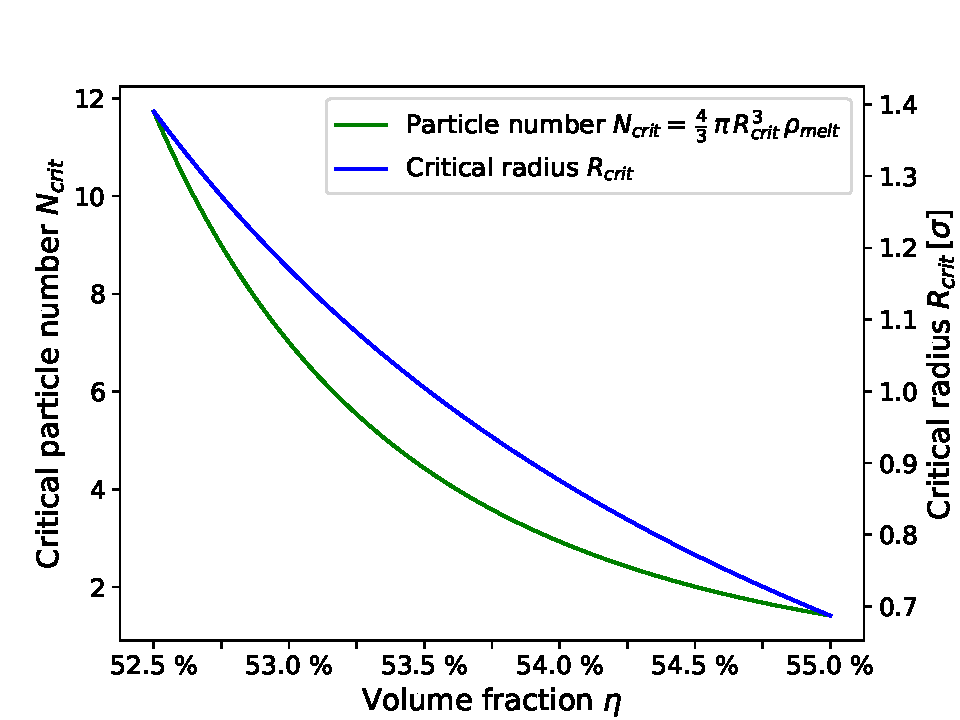
\includegraphics[width=0.53 \linewidth]{CNT_radius.pdf}
\caption[Critical radius in the metastable regime]{Critical radius $R_{\text{crit.}}$ calculated from CNT depending on the volume fraction $\eta$. The critical radius obtained by our calculation is rather small, but when using the chemical potential calculated by Schilling or Filion\cite{Schilling2011, Filion2010a}, the critical cluster size is of the order $N \approx 50$ at intermediate metastable volume fractions, corresponding closer to typical fluctuations of the largest cluster found in simulations.}
\label{fig:r_crit}
\end{figure}

\section{Computer precision and chaotic behavior}
\label{sec:precision}
The finite floating point precision impacts the outcome of the simulation as it constitutes a many body problem with chaotic behavior. In this section it is shown that, for example, even smallest variations of positions lead to radical changes of the simulation after a certain number of steps. It is used to emphasize the importance of rigorously saving the simulation state if it is supposed to be restarted from a file, or with changing measurement intervals. Also, it reminds us that the numerical simulation only is an approximation that never follows the phase space trajectories of the true system.\\

The exponential growth of induced variations in a chaotic system can be visualized by comparing a reference simulation with a perturbed one. In \autoref{fig:chaotic_behavior}, the mean of the squared displacements of all particles is recorded between such a pair of simulations. The perturbation consists of a slight push of $10^{-10} \sigma$ to one particle's position, which is comparable to missing some floating point precision during saving and loading.\\

\begin{figure}[h]
\centering
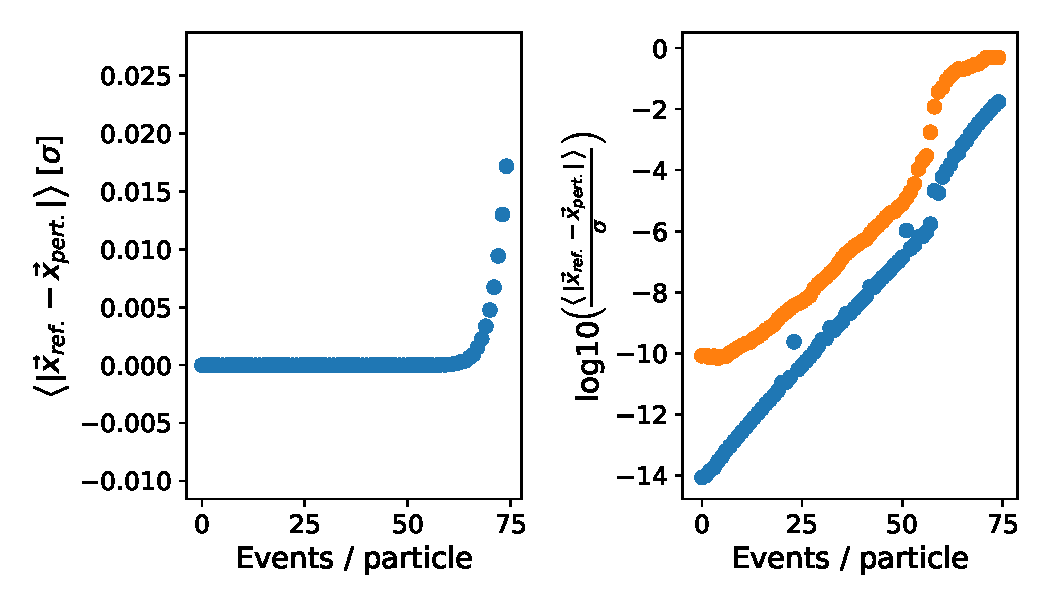
\includegraphics[width=0.6 \linewidth]{perturbation.pdf}
\caption[Exponential growth of perturbations in chaotic system]{Mean difference of particle positions in the reference and perturbed simulation. The blue lines show the same data, while the orange curve shows the maximum deviation present at each step. For comparison with datasets using the system time $\delta t$ as units, a rough conversion is given by $T \approx \text{(\#steps)} \cdot \frac{1 \delta t}{60 \text{steps}}$, where a step is defined as one event execution per particle.\\ The maximum deviation first consists only of the initial perturbation but then increases similar to the mean deviation.}
\label{fig:chaotic_behavior}
\end{figure}

The assumption, that the simulations remain the same to a certain point and then suddenly diverge, can be made when observing only the left side. However, in the logarithmic representation we see that the perturbation actually grows exponentially as long as it is small. It deviates from this exponential growth at the point when reference and perturbed simulation become more or less independent of each other.\\
The small bumps seemed to be an artifact of the periodic boundary conditions but on a second look this was not validated. What causes these deviations therefore remains hidden.\\

The challenge this behavior poses is that any perturbation pushes the system to a completely different trajectory. In the context of EDMD simulations, we can examine the case when a measurement of some quantity is performed. For this purpose, all particles have to be propagated to the global time. To not perturb the system with this extra calculations, an exact copy of the particle positions has to be saved prior to the measurement. Following it, this copy is then used to restore the unperturbed system.\\ 
Similarly recalculating an event for the FEL at some point of time is not possible as the outcome will vary in the last digits. For this reason, it becomes necessary to save all precalculated events of the simulation in order to be able to restart it from a file.\\
However, facing this challenge makes it possible, for example, to resimulate an interesting part of a trajectory from some saved checkpoint with a higher measurement frequency to resolve more details. 
\newpage
\section{Comparison to real world experiments} 
\label{sec:comparison}
Starting in 1986 with the experiments by Pusey and Megen\cite{Pusey1986}, hard sphere like systems have been synthesized in the laboratory. Today, a large variety of them is known, but further systems are being developed aiming at controlling stability and sphere size as well as reducing the possible impact of charges on top of the spheres because the Coulomb interaction alters the behavior of the system. Common to all is, that the hard spheres are suspended in some fluid and that usually its mass density has to be matched to the mass density of the hard spheres to prevent sedimentation. An exception to this may be nucleation experiments that have been done in space without gravity. See Doherty et al. 1998\cite{Doherty1998}. Further, it is necessary for optical measurements to match the refractive index of the fluid and the spheres because otherwise the probe becomes opaque.\\

The absence of the bath in simple hard sphere simulations constitutes a large difference to those experiments in the laboratory. It has been argued, that this only introduces a difference of the time scale which can be compensated by using the characteristic diffusion time as the unit of time. However, a discussion on the possibility of hydrodynamic effects changing the behavior of the laboratory system compared to simulations is ongoing at the moment. See Radu and Schilling 2014\cite{Radu2014} compared to Fiorucci et al. 2020\cite{Fiorucci2020a}.\\
A more subtle detail is the missing mode spectrum of the suspending fluid within the cavities between the dispersed spheres. However, showing its importance requires further investigation.\\ 
Nevertheless, simulations probably could approximate the real world more accurate by including the suspending fluid, but the proliferation of particles raises calculation times by orders of magnitude.\\

A further difference is given by the spatial geometry and extent of the simulation. The geometry in simulations is often chosen with the unphysical setup of periodic boundary conditions (PBC) which are used to avoid surface effects. The impact of this geometry is studied well because the setup is very commonly used. \\ 
Concerning the spatial extent, simulations are mostly confined to very small systems in comparison to experimental setups leading to a further major difference between the measurement geometries. While the experimentalists usually probe a large continuous volume of hard spheres in a suspending fluid, the theorists mostly use many disjunct volumes, as each subvolume can be processed by a single CPU, making simple parallelization of the calculations possible.\\

Measurement techniques, to determine the nucleation state of the experiment, also vary. Light scattering on the growing crystal planes is often used in experiments to measure the crystallinity of a sample because the information of each single particle position is most of the time not accessible. Subsequently, a nucleation time can be defined by when an overall crystallinity is obtained. In comparison, theorists have access to all positions, but no simple measurement like light scattering available. Instead, they use a variety of cluster finding algorithms to determine crystalline local structures. The nucleation time then can be defined by the mean waiting time until a stable crystalline phase is found, for example, Filion et al. 2010\cite{Filion2010a}.\\ 

A discussion on possible definitions of the nucleation time is done in \autoref{sec:nucleation_times}. Furthermore, we will discuss the nucleation behavior of the common simulation geometry in \autoref{sec:induction_time_expectation} and the corresponding one for the infinitely large volume in \autoref{sec:inf_vol_limit_nuc_rate}. Finally, this leads to a possible explanation of the discrepancy between the nucleation rates measured in simulations and laboratory based experiments.

\FloatBarrier
